

PDRと他の情報を使ってライブラリを作成する上で,
どのような状況や環境が存在し補正に利用できるのかその具体的な例を考える必要がある.
例えば大学内や病院などのWi-FiのAPが多く設置されている場所では,
Wi-Fiの電波強度を利用した位置推定が有効である.
他の例として展示会場や大きなアトリウムなどの広い開放空間が考えられる.
このような場所ではWi-FiのAPの配置が難しく,
信号のカバレッジが不均一になりやすくWi-Fiを利用した位置推定は難しい.
このような場所の場合BLEビーコンを配置してその電波強度を利用した位置推定が有効である.
また2章で示したように\cite{pdr-wifi}\cite{pdr-ble}などのPDRと電波を利用した推定に関する研究は盛んに行われている.
このように電波を使った手法は多くの場所で有効であり,補正に利用可能な情報として重要度が高い.
そのため本ライブラリにおいても採用を行う.
他に補正に利用可能な情報としてフロアマップ情報がある.
フロアマップ情報は多くの場所で比較的入手が容易だと思われる.
そのため本ライブラリにおいても採用を行う.

磁気やカメラなどの情報は,磁気はデータが繊細であり電波と比べると補正に利用する難易度が高い,
カメラはプライバシーなどの問題があり本ライブラリの基礎段階においてこれらを採用しない.
また気圧センサは基礎段階として3次元空間を推定対象としないため採用しない.

本ライブラリの補正アルゴリズム実装の検討および,その有効性の検証においてxDR Challenge 2023\cite{xdr}の環境を用いる.
xDR Challenge 2023 はPDRベンチマーク委員会が主催する屋内位置推定の精度を競うコンテストである.
このコンテストでは主催者が参加者に対して複数の訓練データを提供する.
被験者は腰にスマートフォンをつけた状態で,LiDARと呼ばれる距離測定技術を搭載したハンドヘルドLiDARを持ちBLEビーコンが配置された高速道路のサービスエリア内を歩く.
この過程で取得されたデータが訓練データとして提供される.
LiDARからは歩行者のフロアマップにおける歩行者の初期位置,終了位置,移動経路のデータが提供される.
LiDARは光を使って物体や壁までの距離を精密に測定できる技術であり,
このコンテストではLiDARから得られる提供データを正解軌跡として扱っている.
スマートフォンからは加速度,角速度,地磁気,各BLEビーコンのAP情報と受信電波強度が提供される.
フロアマップ情報,各ビーコンのフロアマップにおける基地局の位置情報は事前にコンテスト主催者側によって提供される.
そしてこの提供されたデータを基にコンテスト参加者は独自の推定アルゴリズムの開発を行い位置推定を行う.
本番で与えられるスコアを付けるためデータは訓練データと同様のフロアマップのデータが提供されるが,
LiDARからのデータは初期位置,初期姿勢,終了位置,終了姿勢のみが提供され,それ以外の情報を使って歩行者の移動軌跡を推定する.
xDR Challenge 2023の環境は,フロアマップ情報,各ビーコンの情報,スマートフォンからのセンサデータが提供されている.
そのためPDRと他の情報を使用した補正が可能であり,本ライブラリの要求仕様に適合している.
またライブラリを用いた処理の結果どのような補正の効果が得られるのかを検証する必要がある.
xDR Challenge 2023の環境は後述する評価システムが確立されており,本ライブラリの有効性を検証する環境が整備されている.
よってこの環境を基に補正アルゴリズム実装の検討および有効性の検証を行う.



\begin{figure}[ht]
	\centering
	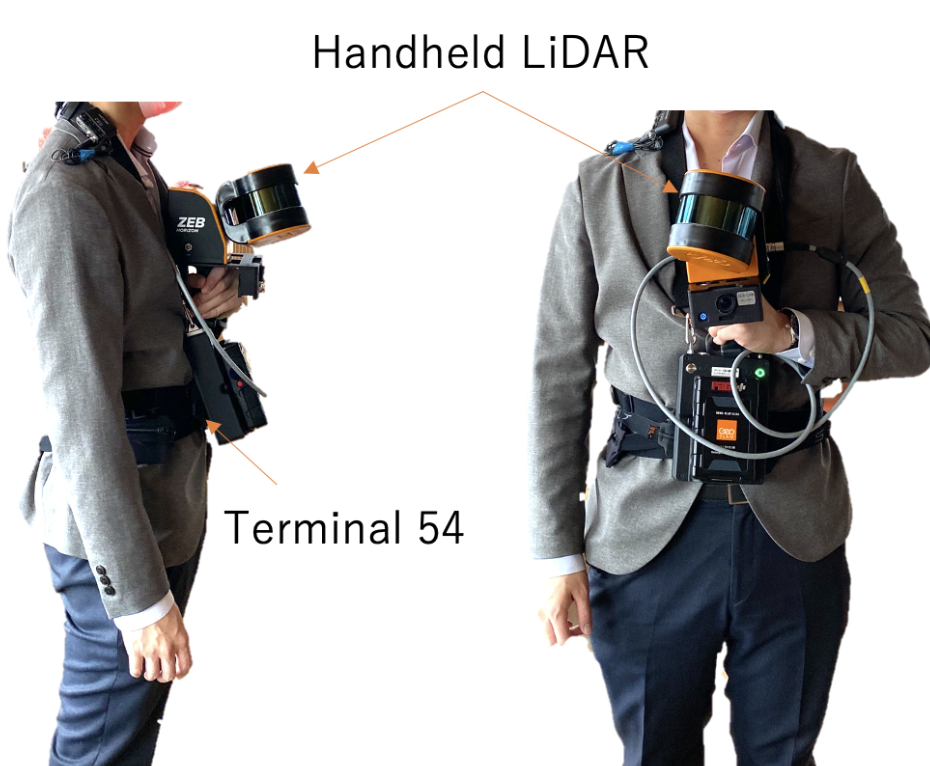
\includegraphics[width=130mm]{image/lidar.jpg}
	\caption{歩行者の装着器具}    \label{fig:step_detect}
\end{figure}
